
\section*{Общая характеристика работы}

\newcommand{\actuality}{\underline{\textbf{\actualityTXT}}}
\newcommand{\progress}{\underline{\textbf{\progressTXT}}}
\newcommand{\aim}{\underline{{\textbf\aimTXT}}}
\newcommand{\tasks}{\underline{\textbf{\tasksTXT}}}
\newcommand{\novelty}{\underline{\textbf{\noveltyTXT}}}
\newcommand{\influence}{\underline{\textbf{\influenceTXT}}}
\newcommand{\methods}{\underline{\textbf{\methodsTXT}}}
\newcommand{\defpositions}{\underline{\textbf{\defpositionsTXT}}}
\newcommand{\reliability}{\underline{\textbf{\reliabilityTXT}}}
\newcommand{\probation}{\underline{\textbf{\probationTXT}}}
\newcommand{\contribution}{\underline{\textbf{\contributionTXT}}}
\newcommand{\publications}{\underline{\textbf{\publicationsTXT}}}


{\actuality} 
Ежедневное усложнение технических объектов управления (ОУ) и все большее внедрение средств автоматизации в различные сферы человеческой деятельности приводят к необходимости развития средств интеллектуального управления. Такие средства интеллектуального управления должны быть применимы в условиях параметрических и структурных неопределенностей. Классические методы теории автоматического управления, хоть и являются достаточно изученными и широко применимыми, имеют целый ряд неустранимых недостатков. К примеру, регуляторы с постоянными настройками не обеспечивают должного качества в условиях, когда параметры ОУ меняются во время функционирования или имеют значительный разброс для разных копий ОУ. К тому же, современные ОУ - зачастую нелинейные объекты с весьма приблизительным математическим описанием. Задача идентификации ОУ также бывает нетривиальной из-за наличия помех в процессе реального функционирования. Решение данных проблем связывают с развитием интеллектуальных систем управления в основе которых лежат искусственные нейронные сети.

С конца 1980-х начала 1990-х активное развитие получила группа алгоритмов обучения с подкреплением (англ. reinforcement learning - RL), которая является одним из разделов машинного обучения (англ. machine learning). После некоторого затишья, в 2013 году, учеными компании DeepMind был разработан модифицированный алгоритм обучения с подкреплением, в основе которого лежали глубокие искусственные нейронные сети, который показал блестящий результат в решении управлении игроком для игр Atari []. Затем, в 2016, учеными той же компании была разработана система на основе обучения с подкреплением для игры в Го, которая оказалась сильней лучших игроков на тот момент []. В 2017 году учеными некоммерческой компании OpenAI разработан бот, также на основе обучения с подкреплением, для игры в Dota 2 в модификации 1 на 1. Данный класс игр с неполной информации казался непосильным рубежом для алгоритмов искусственного интеллекта, однако этот бот обыграл лучшего игрока. В основе метода обучения с подкреплением лежит идея, заимствованная из живой природы, которая позволяет организмам приспосабливаться к изменяющимся условиям среды, а именно получение сигнала подкрепления, который свидетельствует о том, хорошо ли система функционирует. К примеру, хищник, который умеет хорошо охотится, получит подкрепление в виде пойманной жертвы, и наоборот, недостаточно "умная" жертва получит отрицательное подкрепление в виде ранения или смерти, если её догонит хищник. Агент, функционирующий по методу обучения с подкреплением получает сигнал подкрепления от среды, и, в зависимости от этого сигнала, меняет стратегию своего поведения.

Первой особенностью данного метода является то, что система управления не обладает никакой информации о среде и получает все данные только в результате обучения, в котором происходит взаимодействие со средой. Второй особенностью метода обучения с подкреплением является формирование управляющих воздействий с учетом информации о подкреплении, которое будет получено в будущем.


% {\progress} 
% Этот раздел должен быть отдельным структурным элементом по
% ГОСТ, но он, как правило, включается в описание актуальности
% темы. Нужен он отдельным структурынм элемементом или нет ---
% смотрите другие диссертации вашего совета, скорее всего не нужен.

{\aim} данной работы является разработка нейросетевого метода интеллектуального управления, базирующегося на принципах обучения с подкреплением и обеспечивающего возможность мультиагентного взаимодействия.

Для~достижения поставленной цели необходимо было решить следующие {\tasks}:
\begin{enumerate}
	\item Анализ нейросетевых методов управления техническими объектами
	\item Разработка структуры модели на основе нейросетевого обучения с подркеплением для автоматического управления техническими объектами
	\item Разработка програмного обеспечения, реализующего нейросетевой метод управления техническими объектами на основе обучения с подкреплением

  \item Разработка структурной схемы нейросетевой Актор-Критик САУ.
  \item Разработка структурной схемы кооперативного взаимодействия агентов.
  \item Разработка программных средств для функционирования нейросетевой Актор-Критик САУ и сред функционирования агентов.
  \item Выработка рекомендаций по настройке параметров обучения нейросетевой Актор-Критик САУ.
  \item Апробация разработанного метода управления в задачах управления нелинейными ОУ.
\end{enumerate}


{\novelty}
\begin{enumerate}
  \item Впервые получена структура нейросетевая Актор-Критик САУ на основе обучения с подкреплением, которая позволяет формировать управляющее воздействие на ОУ в соответствии с выбранным криетрием функционирования в условиях неизвестных или изменяющихся свойств ОУ.
  \item Впервые получена и применена Кооперативная нейросетевая Актор-Критик САУ на основе обучения с подкреплением, которая позволяет в процессе обучения самостоятельно выработать метод кооперации.
  \item Модифицированный алгоритм обучения нейронных сетей Актора и Критика, который обеспечивает устойчивость процесса обучения, а также быстроту сходимости.
  \item Применен нейросетевой Актор-Критик метод для управления погрузчиком на модели автоматизированного склада
\end{enumerate}

{\influence} Предлагаемый метод может быть использован при разработке интеллектуальных систем управления для ОУ без информации о структуре и параметрах математической модели.

{\methods} В работе были применены методы системного анализа, математического моделирования, теории управления, теории оптимизации, теории нейронных сетей, теории вероятности.

{\defpositions}
\begin{enumerate}
	\item Метод синтеза нейросетевой Актор-Критик САУ на основе обучения с подкреплением для ОУ с неизвестными или изменяющимися свойствами
	\item Нейросетевая Актор-Критик САУ способная управлять ОУ для выполнения одновременно нескольких задач
	\item Кооперативная нейросетевая Актор-Критик САУ на основе модифицированного алгоритма позволяет в процессе обучения самостоятельно выработать метод кооперации.
	\item Кооперативная нейросетевая Актор-Критик САУ в задаче управления несколькими погрузчиками на автоматическом складе
\end{enumerate}

{\reliability} полученных результатов обеспечивается \ldots \ Результаты находятся в соответствии с результатами, полученными другими авторами.


{\probation}
Основные результаты работы докладывались~на:
перечисление основных конференций, симпозиумов и~т.\:п.

{\contribution} Автором непосредственно получены все основные результаты работы: разработана структуры Актор-Критик САУ, Кооперативной Актор-Критик САУ, написаны программы <<Агент Актор-Критик>>, <<Агента Кооперативный Актор-Критик>>.

%\publications\ Основные результаты по теме диссертации изложены в ХХ печатных изданиях~\cite{Sokolov,Gaidaenko,Lermontov,Management},
%Х из которых изданы в журналах, рекомендованных ВАК~\cite{Sokolov,Gaidaenko}, 
%ХХ --- в тезисах докладов~\cite{Lermontov,Management}.

\ifnumequal{\value{bibliosel}}{0}{% Встроенная реализация с загрузкой файла через движок bibtex8
    \publications\ Основные результаты по теме диссертации изложены в XX печатных изданиях, 
    X из которых изданы в журналах, рекомендованных ВАК, 
    X "--- в тезисах докладов.%
}{% Реализация пакетом biblatex через движок biber
%Сделана отдельная секция, чтобы не отображались в списке цитированных материалов
    \begin{refsection}[vak,papers,conf]% Подсчет и нумерация авторских работ. Засчитываются только те, которые были прописаны внутри \nocite{}.
        %Чтобы сменить порядок разделов в сгрупированном списке литературы необходимо перетасовать следующие три строчки, а также команды в разделе \newcommand*{\insertbiblioauthorgrouped} в файле biblio/biblatex.tex
        \printbibliography[heading=countauthorvak, env=countauthorvak, keyword=biblioauthorvak, section=1]%
        \printbibliography[heading=countauthorconf, env=countauthorconf, keyword=biblioauthorconf, section=1]%
        \printbibliography[heading=countauthornotvak, env=countauthornotvak, keyword=biblioauthornotvak, section=1]%
        \printbibliography[heading=countauthor, env=countauthor, keyword=biblioauthor, section=1]%
        \nocite{%Порядок перечисления в этом блоке определяет порядок вывода в списке публикаций автора
                vakbib1,vakbib2,%
                confbib1,confbib2,%
                bib1,bib2,%
        }%
        \publications\ Основные результаты по теме диссертации изложены в \arabic{citeauthor} печатных изданиях, 
        \arabic{citeauthorvak} из которых изданы в журналах, рекомендованных ВАК, 
        \arabic{citeauthorconf} "--- в тезисах докладов.
    \end{refsection}
    \begin{refsection}[vak,papers,conf]%Блок, позволяющий отобрать из всех работ автора наиболее значимые, и только их вывести в автореферате, но считать в блоке выше общее число работ
        \printbibliography[heading=countauthorvak, env=countauthorvak, keyword=biblioauthorvak, section=2]%
        \printbibliography[heading=countauthornotvak, env=countauthornotvak, keyword=biblioauthornotvak, section=2]%
        \printbibliography[heading=countauthorconf, env=countauthorconf, keyword=biblioauthorconf, section=2]%
        \printbibliography[heading=countauthor, env=countauthor, keyword=biblioauthor, section=2]%
        \nocite{vakbib2}%vak
        \nocite{bib1}%notvak
        \nocite{confbib1}%conf
    \end{refsection}
}
При использовании пакета \verb!biblatex! для автоматического подсчёта
количества публикаций автора по теме диссертации, необходимо
их здесь перечислить с использованием команды \verb!\nocite!.
    

 % Характеристика работы по структуре во введении и в автореферате не отличается (ГОСТ Р 7.0.11, пункты 5.3.1 и 9.2.1), потому её загружаем из одного и того же внешнего файла, предварительно задав форму выделения некоторым параметрам

%Диссертационная работа была выполнена при поддержке грантов ...

%\underline{\textbf{Объем и структура работы.}} Диссертация состоит из~введения, четырех глав, заключения и~приложения. Полный объем диссертации \textbf{ХХХ}~страниц текста с~\textbf{ХХ}~рисунками и~5~таблицами. Список литературы содержит \textbf{ХХX}~наименование.

%\newpage
\section*{Содержание работы}
Во \underline{\textbf{введении}} обосновывается актуальность
исследований, проводимых в рамках данной диссертационной работы,
приводится обзор научной литературы по изучаемой проблеме,
формулируется цель, ставятся задачи работы, излагается научная новизна
и практическая значимость представляемой работы.


\underline{\textbf{Первая глава}} посвящена обзору современных методов обучения с подкреплением, приведен обзор различных алгоритмов.

При постановке задач обучения с подкреплением (Reinforcement learning, коротко RL) исследуемую систему условно разделяют на два блока: агент и динамический процесс или среда. Агент - структурно автономная система, которая в процессе функционирования системы производит наблюдения, выбирает действие и применяет это действие на среду, меняя её состояние. Схематичная визуализация взаимодействия показана на рисунке \ref{img:rl} Цель агента - выбирать адекватные задаче действия.

\begin{figure}[ht] 
	\center
	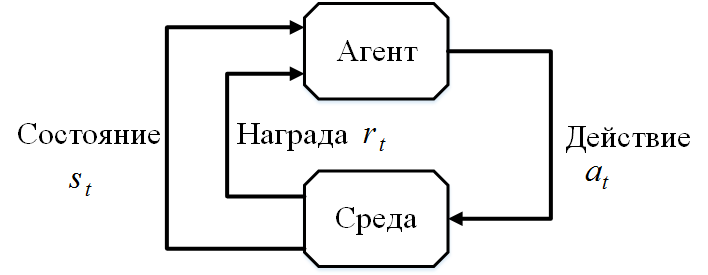
\includegraphics [scale=0.5] {rl}
	\caption{Схема взаимодействия агента со средой} 
	\label{img:rl}  
\end{figure}

В процессе обучения агент принимает специальный скалярный сигнал от среды - подкрепление. Этот сигнал показывает, насколько хорошо агент выполняет поставленную задачу. Обычно этот сигнал связывается только с теми событиями, которые кардинально влияют на процесс: успешное выполнение части задачи, задачи целиком (сигнал награды) или же наоборот, критическая ошибка агента (сигнал штрафа), приведшая к драматическим событиям. Именно этот аспект отличает обучение с подкреплением от обучения с учителем (supervised learning), при котором предоставляются пары <<входные данные - ответ>>. 


В произвольный момент времени $ t_i $ агент принимает состояние среды $ s_i\in S $, где $ S $ некоторое конечное множество возможных состояний внешней среды, и, базируясь на этой информации, вырабатывает определенное воздействие на среду $ a_i\in A(s_i) $, где $ A(s_i) $ конечное множество действий, которые могут быть оказаны на среду в состоянии $ s_i $. Данное воздействие $ a_i $ переводит среду в состояние $ s_{i+1} $, а агент получает вознаграждение $ r_i $. Агент в процессе обучения должен выработать такую стратегию $ \pi: S \rightarrow A $, чтобы максимизировать $ R_i $ - суммарную величину всех подкреплений.

Различают два типа задач обучения с подкреплением:
\begin{itemize}
	\item задачи с терминальным состоянием - эпизодические;
	\item задачи без терминального состояния - непрерывные.
\end{itemize}

Для эпизодической задачи $ R_i $ определяется как:
\begin{equation}
\label{eq:1_1p1}
\begin{alignedat}{2}
R_i=r_{i+1} + r_{i+2} + \cdots + r_N = \sum \limits_{k=i}^{N}r_{i+1+k} \end{alignedat}
\end{equation}
где $ i $ - номер шага, а $ N $ - количество шагов в эпизоде.

В отличии от эпизодических задач, где эпизод состоит из конечного числа шагов и суммарная величина подкрепления всегда может быть ограничена некоторой максимальной величиной, непрерывные задачи могут иметь $ R_i $ стремящееся к бесконечности. Для таких случаев применяют выражение:
Для эпизодической задачи $ R_i $ определяется как:
\begin{equation}
\label{eq:1_1p2}
\begin{alignedat}{2}
R_i=r_{i+1} + \gamma \cdot r_{i+2} + \gamma^2 \cdot r_{i+3} + \cdots = \sum \limits_{k=0}^{\infty}\gamma^k \cdot r_{i+1+k}
\end{alignedat}
\end{equation}
где $ \gamma \in [0, 1]$ - коэффициент дисконтирования подкрепления, который обеспечивает сходимость суммарной величины подкрепления.  
Параметр дисконтирования взвешивает значения подкрепления, полученные в прошлом относительно новых. Чем ближе $ \gamma $ к единице, тем больше агентом принимаются во внимание новые сигналы от среды, а если $ \gamma = 0 $, то все будущие сигналы подкрепления никак не будут учтены. 


\underline{\textbf{Вторая глава}} посвящена исследованию 

В подходе с обучением с подкреплением целью функционирования агента является максимизация целевой функции, который представляет собой суммарную величину награды - подкрепления. Такого типа управление относится к классу систем экстремального управления (СЭУ).


Системы экстремального управления относят к классу адаптивных систем, такие системы отличаются автоматическим выбором режима управления, при котором поддерживается минимальное или максимальное значение некой целевой функции. 

\begin{figure}[ht] 
	\center
	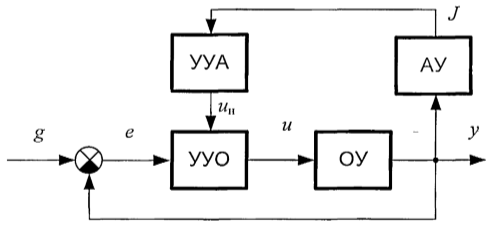
\includegraphics [scale=0.5] {seu_21}
	\caption{Структурная схема СЭУ} 
	\label{img:seu_21}  
\end{figure}

%\newpage
%============================================================================================================================

С помощью метода Актор-Критик и обучения с подкреплением разработана обобщенная структурная схема Актор-Критик САУ, изображенная на рисунке ~\ref{img:ac_struct}, а также алгоритмы функционирования системы
\begin{figure}[ht] 
	\center
	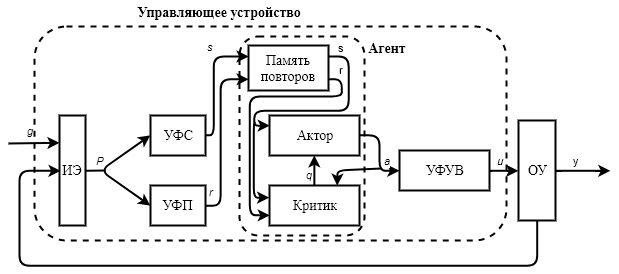
\includegraphics [scale=0.5] {ac_struct}
	\caption{Структурная схема Актор-Критик САУ} 
	\label{img:ac_struct}  
\end{figure}


Объект управления должен обладать свойствами частично наблюдаемого марковского процесса (POMDP)

Целью функционирования импульсного элемента является дискретизация поступающего на вход сигнала с шагом $\tau_{\text{УУ}}$, который является параметром настройки УУ. ИЭ отвечает за формирование вектора дискретных сигналов $\bar{P}[k]$, который вектор поступает на входы УФС и УФП. Вектор $\bar{P}[k]$ состоит из $N_{\text{ОУ}}$ элементов, где $N_{\text{ОУ}}$ количество переменных состояния ОУ.

Блок УФС отвечает за создание вектора состояний $s[k]$, который поступает на вход Актору и Критику. Данный вектор состоит из квантованных и нормализованных к масштабу [-1, 1] значений вектора $\bar{P}[k]$. Нормализация к данному масштабу объяснятся отраслевым стандартом.


УФП отвечает за выработку сигнала подкрепления $ r[k] $ из вектора дискретных значений $ \bar{P}[k] $ c помощью функции $ f $:
$$
r[k] = f(p_1[k]), p_2[k]), p_{N_p}[k])).
$$

Данная функция является параметром настройки блока УФП, и выбирается в зависимости от задачи. Если целью функционирования системы является поддержание некого постоянного значения $ y_{\text{зад}} $, то функция вычисления сигнала подкрепления может иметь вид:

$$
f(y) = -(y-y_{\text{зад}})^2.
$$

\noindent Такой вид функции обеспечивает максимальный сигнал подкрепления (равный 0) только в том случае, если значение выходного сигнала совпадет с  $ y_{\text{зад}} $.

Когда целью функционирования системы является достижение единовременное некоторой цели, например передвижение кибер-физической системы из одного положение в другое, то функций расчета подкрепления становится система эвристических правил. Например, задачей мобильного робота является перемещение из положения $ A $ в положение $ A^* $, а положение самого робота обозначается $ A_r $. Функция $ D_{(A^*, A_r)} $ расчитывает расстояние между мобильным роботом и целевой точкой. Функция расчета сигнала подкрепления может иметь следующий вид:

$$
r[k] = 
\begin{cases}
1, \: \text{если} \: D_{(A^*, A_r)}=0; \\
0.1, \: \text{если} \: D_{(A^*, A_r)}[k] < D_{(A^*, A_r)}[k-1]; \\
-0.1 \: \text{иначе}.
\end{cases}
$$

\noindent В данной функции отрицательное подкрепление или штраф агент получает в случае бездействия, когда расстояние до цели не уменьшается, награждается в случае сближения с целью, и самый большой сигнал подкрепления агент получает в случае попадания в цель.

На практике вводится некоторая отсечка $ T_{\text{сближ}} $ для расчета сигнала подкрепления в случае сближения робота с целью, если величина сближения  меньше этой отсечки, то награда не назначается. Это делается для исключения колебаний сигнала подкрепления. Дополнительно вводится отсечка достижения робота цели $ T_{\text{цели}} $. Если робот слишком далеко переместился от цели, дальше чем $ T_{\text{откл}} $, то назначается штраф. После введения вышеперечисленных отсечек функция расчета подкрепления принимает следующий вид:

$$
r[k] = \begin{cases}
1, \: \text{если} \: D_{(A^*, A_r)} < T_{\text{цели}}; \\
0.1, \: \text{если} \: D_{(A^*, A_r)}[k-1] - D_{(A^*, A_r)}[k] > T_{\text{сближ}}; \\
-1 \: D_{(A^*, A_r)} > T_{\text{откл}};\\
-0.1 \: \text{иначе}.
\end{cases}
$$

\noindent Данные отсечки являются параметрами настройки блока УФП. Если сигнал подкрепления равен 1 или -1 то эпизод заканчивается победой или поражением соответственно.

"Агент" является блоком, реализующим алгоритм, в основе функционирования которого лежит метод Актор-Критик. Данный метод был выбран на основе анализа, приведенного в главе \ref{subsect1_3_6}.

На вход данного блока подается вектор состояния $s[k]$ и сигнал подкрепления $r[k]$. Блок "Агент" состоит из трёх подблоков: Актора, Критика и блока повторов. Актор отвечает за формирование сигнала управления и Критик за анализ качества управления. Блок повторов содержит в себе информацию о предыдущих результатах взаимодействия Актора, Критика и средой. У <<Агента>> есть два режима функционирования:
\begin{enumerate}
	\item Обучение. Задействованы и Актор и Критик.
	\item Предсказание. Работает только Актор.
\end{enumerate} 

Параметрами настройки блока <<Агент>> являются:
\begin{itemize}
	\item $ N_s $ - количество состояний $s[k]$;
	\item $ N_a $ - количество параметров во множестве воздействий на ОУ $ A $;
	\item $ \gamma $ - коэффициент дисконтирования сигнала подкрепления;
	\item $ \Delta $ - коэффициент скорости обучения (learning rate);
	\item $ f_{\epsilon} $ - закон изменения коэффициента исследования;
	\item $ N_R $ - количество элементов в памяти повторов;
	\item также в качестве параметров настройки блока выступают количество слоев ИНС и количество нейронов в каждом из них.
\end{itemize}

Подблоки Актор и Критик использует для аппроксимации своих функций глубокие нейронне сети (DNN - deep neural network), настраиваемыми параметрами которых являются $ \theta_A $ и $ \theta_K $ соответственно. Метод, которым производится обучение Актора и Критика называется DDPG (Deep deterministic policy gradient). 

Функция Критика аппроксимируется через минимизацию квадратичной ошибки временной разности:

$$
L(\theta_K) = (r_{i+1} + \gamma Q(s_{i+1}, \pi(s_{i+1}|\theta_A)|\theta_K) - Q(s_i, a_i|\theta_K))^2
$$

$$
y_i = r_i + \gamma Q'(s_{i + 1}, \mu'(s_{i+1}|\theta^{\mu'})|\theta^{Q'})
$$

$$
L = \frac{1}{N} \sum_{i} (y_i - Q(s_i, a_i | \theta^{Q})^2) 
$$

$$
\nabla_{\theta^{\mu}} \mu \approx \mathbb{E}_{\mu'} \big [ \nabla_{a} Q(s, a|\theta^{Q})|_{s=s_t,a=\mu(s_t)} \nabla_{\theta^{\mu}} \mu(s|\theta^{\mu})|_{s=s_t} \big ]
$$

Веса нейронной сети Актора настраиваются по направлению градиентов $ \Delta Q_{\theta_A} $ по следующей формуле:

$$ 
\Delta \theta_A = \Delta
$$

$$
a[k] = 
\begin{cases}
a^*[k], \: \text{если} \: e \geq \epsilon  \\
a_t, \: t=[rand \cdot N_a]
\end{cases}
$$

Алгоритм работы блока <<Агент>>:
\begin{enumerate}
	\item В соответсвии с () $ \epsilon $ - жадной стратегии выбирается действие $ a_i $ для текущего состояния $ s_i $.
	\item Считывается следующее состояние $ s_{i+1} $ и награда $ r $
	\item Кортеж $ a_i $, $ s_i $, $ s_{i+1} $ и $ r $ записываются в подблок <<Память повторов>>
	\item Считывается N записей из подблока <<Память повторов>>
	\item На основании () производится обновление весов нейронной сети Критика
	\item На основании () производится обновление весов нейронной сети Актора
\end{enumerate}



\underline{\textbf{Третья глава}} посвящена исследованию кооперативного Актор-Критик метода

В \underline{\textbf{четвертой главе}} приведено описание схемы управления погрузчиками на автоматизированном складе

В \underline{\textbf{заключении}} приведены основные результаты работы, которые заключаются в следующем:
%% Согласно ГОСТ Р 7.0.11-2011:
%% 5.3.3 В заключении диссертации излагают итоги выполненного исследования, рекомендации, перспективы дальнейшей разработки темы.
%% 9.2.3 В заключении автореферата диссертации излагают итоги данного исследования, рекомендации и перспективы дальнейшей разработки темы.
\begin{enumerate}
  \item На основе анализа \ldots
  \item Численные исследования показали, что \ldots
  \item Математическое моделирование показало \ldots
  \item Для выполнения поставленных задач был создан \ldots
\end{enumerate}



%\newpage
При использовании пакета \verb!biblatex! список публикаций автора по теме
диссертации формируется в разделе <<\publications>>\ файла
\verb!../common/characteristic.tex!  при помощи команды \verb!\nocite! 

\ifdefmacro{\microtypesetup}{\microtypesetup{protrusion=false}}{} % не рекомендуется применять пакет микротипографики к автоматически генерируемому списку литературы
\ifnumequal{\value{bibliosel}}{0}{% Встроенная реализация с загрузкой файла через движок bibtex8
  \renewcommand{\bibname}{\large \authorbibtitle}
  \nocite{*}
  \insertbiblioauthor           % Подключаем Bib-базы
  %\insertbiblioother   % !!! bibtex не умеет работать с несколькими библиографиями !!!
}{% Реализация пакетом biblatex через движок biber
  \insertbiblioauthor           % Вывод всех работ автора
%  \insertbiblioauthorgrouped    % Вывод всех работ автора, сгруппированных по источникам
%  \insertbiblioauthorimportant  % Вывод наиболее значимых работ автора (определяется в файле characteristic во второй section)
  \insertbiblioother            % Вывод списка литературы, на которую ссылались в тексте автореферата
}
\ifdefmacro{\microtypesetup}{\microtypesetup{protrusion=true}}{}

